\documentclass{beamer}

%
% Choose how your presentation looks.
%
% For more themes, color themes and font themes, see:
% http://deic.uab.es/~iblanes/beamer_gallery/index_by_theme.html
%
\mode<presentation>
{
  \usetheme{default}      % or try Darmstadt, Madrid, Warsaw, ...
  \usecolortheme{default} % or try albatross, beaver, crane, ...
  \usefonttheme{default}  % or try serif, structurebold, ...
  \setbeamertemplate{navigation symbols}{}
  \setbeamertemplate{caption}[numbered]
  \setbeamertemplate{footline}[page number]
  \setbeamercolor{frametitle}{fg=white}
  \setbeamercolor{footline}{fg=black}
} 

\usepackage[english]{babel}
\usepackage[utf8x]{inputenc}
\usepackage{tikz}
\usepackage{listings}
\usepackage{courier}
\usepackage{minted}

\xdefinecolor{darkblue}{rgb}{0.1,0.1,0.7}
\xdefinecolor{dianablue}{rgb}{0.18,0.24,0.31}
\definecolor{commentgreen}{rgb}{0,0.6,0}
\definecolor{stringmauve}{rgb}{0.58,0,0.82}

\lstset{ %
  backgroundcolor=\color{white},      % choose the background color
  basicstyle=\ttfamily\small,         % size of fonts used for the code
  breaklines=true,                    % automatic line breaking only at whitespace
  captionpos=b,                       % sets the caption-position to bottom
  commentstyle=\color{commentgreen},  % comment style
  escapeinside={\%*}{*)},             % if you want to add LaTeX within your code
  keywordstyle=\color{blue},          % keyword style
  stringstyle=\color{stringmauve},    % string literal style
  showstringspaces=false,
  showlines=true
}

\lstdefinelanguage{scala}{
  morekeywords={abstract,case,catch,class,def,%
    do,else,extends,false,final,finally,%
    for,if,implicit,import,match,mixin,%
    new,null,object,override,package,%
    private,protected,requires,return,sealed,%
    super,this,throw,trait,true,try,%
    type,val,var,while,with,yield},
  otherkeywords={=>,<-,<\%,<:,>:,\#,@},
  sensitive=true,
  morecomment=[l]{//},
  morecomment=[n]{/*}{*/},
  morestring=[b]",
  morestring=[b]',
  morestring=[b]"""
}

\title[2016-11-07-rootteam-root4j]{Reading ROOT data in Java and Spark}
\author{Jim Pivarski}
\institute{Princeton -- DIANA}
\date{November 7, 2016}

\begin{document}

\logo{\pgfputat{\pgfxy(0.11, 8)}{\pgfbox[right,base]{\tikz{\filldraw[fill=dianablue, draw=none] (0 cm, 0 cm) rectangle (50 cm, 1 cm);}}}\pgfputat{\pgfxy(0.11, -0.6)}{\pgfbox[right,base]{\tikz{\filldraw[fill=dianablue, draw=none] (0 cm, 0 cm) rectangle (50 cm, 1 cm);}
\includegraphics[height=0.99 cm]{diana-hep-logo.png}\tikz{\filldraw[fill=dianablue, draw=none] (0 cm, 0 cm) rectangle (4.9 cm, 1 cm);}}}}

\begin{frame}
  \titlepage
\end{frame}

\logo{\pgfputat{\pgfxy(0.11, 8)}{\pgfbox[right,base]{\tikz{\filldraw[fill=dianablue, draw=none] (0 cm, 0 cm) rectangle (50 cm, 1 cm);}
\includegraphics[height=1 cm]{diana-hep-logo.png}}}}

% Uncomment these lines for an automatically generated outline.
%\begin{frame}{Outline}
%  \tableofcontents
%\end{frame}

\begin{frame}{Motivation}
\vspace{0.25 cm}
In a physics analysis using Spark {\small (Oliver Gutsche, Matteo Cremonesi, Cristina Mantilla)}, the first step is data access.

\vspace{0.25 cm}
Hard to cross the boundary between ROOT's C++ runtime and Spark's Java Virtual Machine (JVM).

\vspace{0.25 cm}
\begin{uncoverenv}<2->
\textcolor{darkblue}{Four methods considered:}
\begin{enumerate}
\item Convert all data from ROOT to another format (Avro).
\item Access ROOT inside the JVM via JNI.
\item Access ROOT as an external process (pipe or socket).
\item Run PyROOT in PySpark.
\end{enumerate}
\end{uncoverenv}

\vspace{0.25 cm}
\begin{uncoverenv}<3->
The 2016 analysis used option \textcolor{darkblue}{\#1}, but it's not ideal.
\begin{itemize}
\item Separate conversion step before running Spark.
\item Two copies of the data: extra version control and disk usage.
\end{itemize}
\end{uncoverenv}
\end{frame}

\begin{frame}{Previously rejected solution}
\vspace{0.25 cm}
\begin{center}
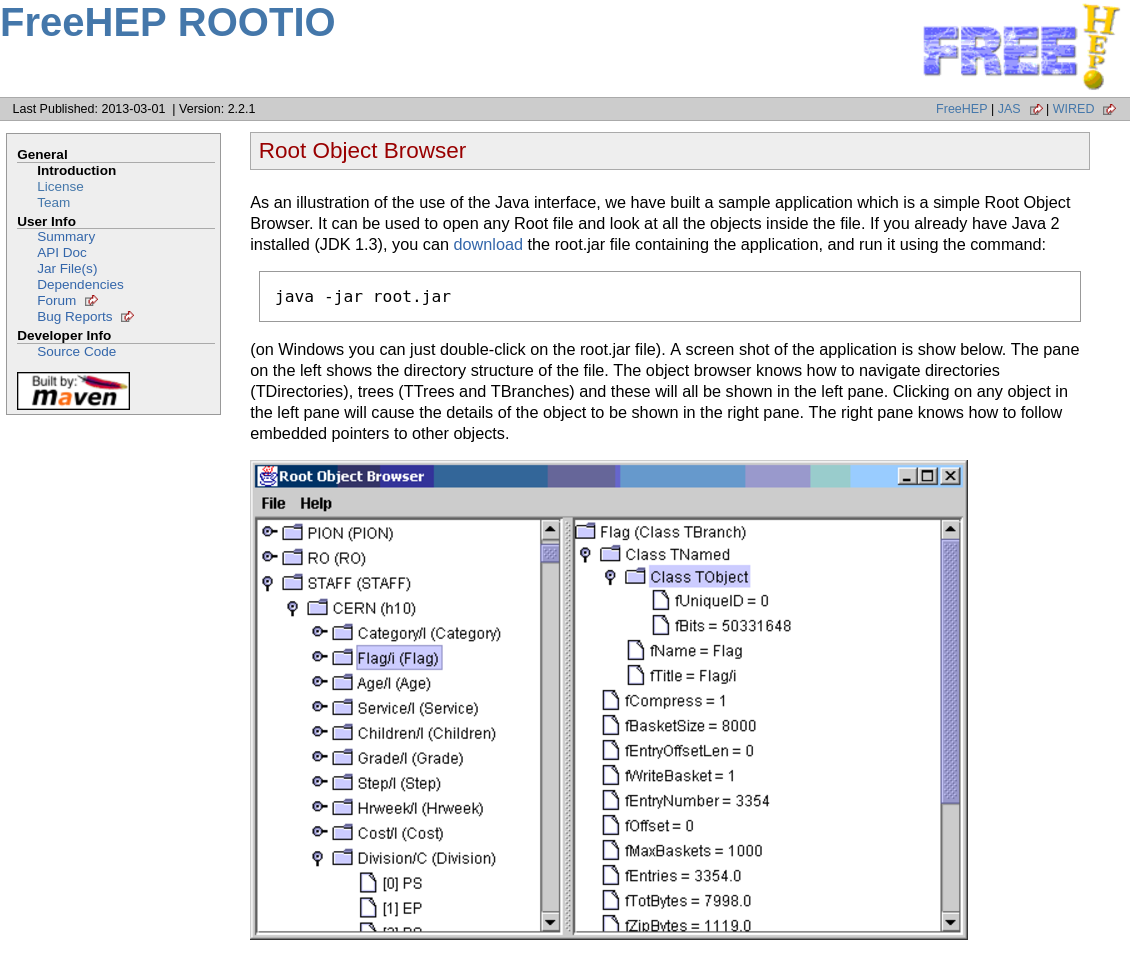
\includegraphics[width=0.9\linewidth]{rootio-screenshot.png}
\end{center}
\end{frame}

\begin{frame}{Previously rejected solution}
\vspace{0.35 cm}
\begin{block}{FreeHEP ROOTIO \scriptsize (\textcolor{blue}{\url{http://java.freehep.org/freehep-rootio/}})}
\vspace{-0.1 cm}
\begin{itemize}
\item Re-implementation of ROOT's I/O in Java.
\item Used as a backend in Java Analysis Studio (JAS).
\item First talks by Tony Johnson in 2001, commits trail off $\sim$2010.
\end{itemize}
\end{block}

\vspace{-0.25 cm}
\begin{uncoverenv}<2->
\begin{block}{Why not?}
\vspace{-0.1 cm}
\begin{itemize}
\item Lack of documentation; high-level interface described on website no longer exists.
\item Immediately failed when presented with recent ROOT file.
\item Can't get in touch with Tony Johnson.
\end{itemize}
\end{block}
\end{uncoverenv}

\vspace{-0.25 cm}
\begin{uncoverenv}<3->
\begin{block}{Why now?}
\vspace{-0.1 cm}
\begin{itemize}
\item I reexamined its low-level interface (direct access to TBranches/TBaskets), and it works!
\item Only 3 minor bug-fixes needed to read complex CMS AOD.
\end{itemize}
\end{block}
\end{uncoverenv}
\end{frame}

\begin{frame}{Why this is a good solution}
\vspace{0.3 cm}
\begin{block}{Reading ROOT files with pure Java code}
\begin{itemize}
\item No intermediate files: version control and extra disk space.
\item No attempt to run two large projects (ROOT and Java) in the same process, which caused hard-to-trace segmentation faults.
\item No passing data through a serialized stream (both solutions \textcolor{darkblue}{\#3} and \textcolor{darkblue}{\#4} on the first page).
\end{itemize}
\end{block}

\vspace{-0.5 cm}
\begin{uncoverenv}<2->
\begin{block}{This particular codebase\vspace{-0.5 cm}}
\renewcommand{\arraystretch}{1.2}
\begin{tabular}{p{0.85\linewidth} c}
& verified? \\\hline
Can read complex structures out of TBasket. & $\surd$ \\
Only small corrections are likely. & $\surd$ \\
Well-organized; class/method names mirror ROOT. & $\surd$ \\
JIT-compiles streamers, rather than generic functions. & $\surd$ \\
Can write objects to ROOT files as well. & \\
Has an embedded XRootD client (HDFS and EOS!). & \\
\end{tabular}
\end{block}
\end{uncoverenv}
\end{frame}

\begin{frame}[fragile]{Project: expose ROOT format to Spark}
\vspace{0.5 cm}
\begin{columns}[t]
\column{0.5\linewidth}
\textcolor{darkblue}{\large \bf root4j}

\vspace{0.1 cm}
\begin{itemize}
\item Fork of original FreeHEP with JAS dependency and GUI components removed.
\item Java, minimal dependencies, built with Maven.
\item LGPL 2.1 (like original).
\end{itemize}

\column{0.5\linewidth}
\textcolor{darkblue}{\large \bf spark-root}

\vspace{0.1 cm}
\begin{itemize}
\item New project, depends on root4j, Hadoop, Spark.
\item Presents ROOT TChain as a Spark DataFrame.
\item Scala, built with SBT.
\item Apache 2.0.
\end{itemize}
\end{columns}

\vspace{1 cm}
\begin{uncoverenv}<2->
\textcolor{darkblue}{\large User would launch Spark like this:}

\small
\begin{minted}{bash}
spark-shell --packages \
    org.diana-hep:spark-root_2.11:1.0.0
\end{minted}

\normalsize
(Spark fetches JAR with dependencies from Maven Central.)
\end{uncoverenv}
\end{frame}

\begin{frame}[fragile]{Example session}
\small
\vspace{0.5 cm}
\begin{minted}{scala}
import org.dianahep.sparkroot._
val df = spark.sqlContext.read.root(
             "hdfs://path/to/files/*.root")

df.printSchema
\end{minted}
\begin{verbatim}
root
 |-- met: float (nullable = false)
 |-- muons: array (nullable = false)
 |    |-- element: struct (containsNull = false)
 |    |    |-- pt: float (nullable = false)
 |    |    |-- eta: float (nullable = false)
 |    |    |-- phi: float (nullable = false)
 |-- jets: array (nullable = false)
 |    |-- element: struct (containsNull = false)
 |    |    |-- pt: float (nullable = false)
 |    |    |-- eta: float (nullable = false)
 |    |    |-- phi: float (nullable = false)
\end{verbatim}
\end{frame}

\begin{frame}[fragile]{Example session}
\small
\begin{verbatim}
df.show
+---------+--------------------+--------------------+
|      met|               muons|                jets|
+---------+--------------------+--------------------+
| 55.59374|[[28.07075,-1.331...|[[194.19714,-2.65...|
|39.440292|                  []|[[93.64958,-0.273...|
|2.1817229|[[5.523367,-0.375...|[[96.09923,0.7058...|
|  80.5822|[[48.910114,-0.17...|[[165.2686,0.2623...|
| 84.43806|                  []|[[51.87823,1.6442...|
| 84.63146|[[33.84279,-0.062...|[[137.74776,-0.45...|
| 393.8167|[[25.402626,-0.66...|[[481.8268,-1.115...|
|  75.0873|                  []|[[144.62373,-2.21...|
|2.6512942|[[6.851382,2.3145...|[[72.08256,-1.713...|
|36.753353|                  []|[[72.7172,-1.3265...|
+---------+--------------------+--------------------+
only showing top 10 rows
\end{verbatim}
\end{frame}

\begin{frame}[fragile]{Example session}
\small
\begin{minted}{scala}
case class LorentzVector(pt: Float, eta: Float)
case class Event(met: Float,
                 muons: Seq[LorentzVector],
                 jets: Seq[LorentzVector])

val rdd = df.as[Event]   // OOP-style interface

import org.dianahep.histogrammar._
import org.dianahep.histogrammar.sparksql._

// RDD plotting
val h1 = rdd.aggregate(
    Bin(100, 0.0, 20.0, {event: Event => event.met}))
    (new Increment, new Combine)

// DataFrame plotting
val h2 = df.histogrammar(Bin(100, 0.0, 20.0, $"met"))
\end{minted}
\end{frame}

\begin{frame}[fragile]{ROOT $\to$ DataFrame features}
\begin{itemize}\setlength{\itemsep}{0.25 cm}
\item SparkSQL examines user's query, optimizes a work plan, and provides data source with the following information:
\begin{itemize}
\item which fields are required (``pruning'');
\item conservative cuts to use as a prefilter (``filtering'').
\end{itemize}

\item Matches perfectly with ROOT's columnar layout: only read pruned branches and execute filter at the source.

\item Since root4j can write (untested) we should also implement 
\begin{verbatim}spark.sqlContext.save.root("filename.root")
\end{verbatim}
to share results back to C++ ROOT.
\end{itemize}
\end{frame}

%% Ignoring the Java startup phase (training HotSpot optimizations), the Java time is 130-200 ns/item and C++ is 80 ns/item.
%% Compression on this branch is 1.09, so Java is 15-25 MB/second and C++ is 40 MB/second.
%% Java is 1.6 to 2 times slower than C++. That makes sense; typical of Java/C++ performance on the benchmarks game.

\end{document}
